% !Mode:: "TeX:UTF-8"
%# -*- coding:utf-8 -*-

%% 南京大学学位论文的示例文档
%% 作者:njuhan: https://github.com/njuHan
%% 源模版repo: https://github.com/njuHan/njuthesis-nju-thesis-template

\documentclass[winfonts,master,twoside]{njuthesis}
%% 审阅模式很重要,命令是下方使用的/blind
%% njuthesis 文档类的可选参数有:
%%   winfonts, linuxfonts, macfonts, adobefonts winfonts 选项使得文档使用Windows 系统提供的字体;linuxfonts 选项使得文档使用Linux 系统提供的字体;macfonts 选项使得文档使用Mac 系统提供的字体;adobefonts 选项使得文档使用Adobe提供的OTF中文字体(需自行下载安转)
%%   phd/master/bachelor 选择博士/硕士/学士论文
%%   twoside 或 oneside 指定排版的文档为双面打印或单面打印格式(twoside会使得chapter 章节从奇数页开始,即纸张的正面开始,因此会出现一些空白的页面)
%%   nobackinfo 取消封二页导师签名信息。注意,按照南大的规定,是需要签名页的。



%%%%%%%%%%%%%%%%%%%%%%%%%%%%%%%%%%%%%%%%%%%%%%%%%%%%%%%%%%%%%%%%%%%%%%%%%%%%%%%
% set up labelformat and labelsep for subfigure 详见: http://www.latexstudio.net/archives/8652.html
\captionsetup[subfigure]{labelformat=simple, labelsep=space}

%%%%%%%%%%%%%%%%%%%%%%%%%%%%%%%%%%%%%%%%%%%%%%%%%%%%%%%%%%%%%%%%%%%%%%%%%%%%%%%
% 设置《国家图书馆封面》的内容,仅博士论文才需要填写

% 设置论文按照《中国图书资料分类法》的分类编号
%\classification{0175.2}
% 设置论文按照《国际十进分类法UDC》的分类编号
% 该编号可在下述网址查询:http://www.udcc.org/udcsummary/php/index.php?lang=chi
%\udc{004.72}
% 国家图书馆封面上的论文标题第一行,不可换行。此属性可选,默认值为通过\title设置的标题。
%\nlctitlea{论文标题第一行}
% 国家图书馆封面上的论文标题第二行,不可换行。此属性可选,默认值为空白。
%\nlctitleb{论文标题第二行}
% 国家图书馆封面上的论文标题第三行,不可换行。此属性可选,默认值为空白。
%\nlctitlec{}
% 导师的单位名称及地址
%\supervisorinfo{南京大学计算机科学与技术系~~南京市汉口路22号~~210093}
% 答辩委员会主席
%\chairman{张三丰~~教授}
% 第一位评阅人
%\reviewera{阳顶天~~教授}
% 第二位评阅人
%\reviewerb{张无忌~~副教授}
% 第三位评阅人
%\reviewerc{黄裳~~教授}
% 第四位评阅人
%\reviewerd{郭靖~~研究员}


%%%%%%%%%%%%%%%%%%%%%%%%%%%%%%%%%%%%%%%%%%%%%%%%%%%%%%%%%%%%%%%%%%%%%%%%%%%%%%%
% 设置论文的中文封面

% 单行论文标题,不可换行
\title{南京大学毕业论文\LaTeX 模板}

% 如果论文标题过长,可以分两行,第一行用\titlea{}定义,第二行用\titleb{}定义,
% 使用以下3行:
%\title{} %用于覆盖单行标题内容为空
%\titlea{长标题第一行}  %第一行标题写这里
%\titleb{长标题第二行用于长标题换行} %第二行标题写这里
% 注意: \title 不能都注释,它用于控制标题选择双行还是单行。\title{}如果内容为空,则编译\titlea{},titleb{}双行标题,否则编译单行标题


% 论文作者姓名
\author{作者}
% 论文作者联系电话
\telphone{xxxx}
% 论文作者电子邮件地址
\email{sample@smail.nju.edu.cn}
% 论文作者学生证号
\studentnum{xxxxxxx}
% 论文作者入学年份(年级)
\grade{2019}
% 论文作者毕业年份(届), 出版授权书的学位年度
\graduateyear{20xx}
% 导师姓名职称
\supervisor{某~~教授,某某~~教授}
% 导师的联系电话
\supervisortelphone{}
% 论文作者的学科与专业方向
\major{工程硕士(软件工程领域)}
% 论文作者的研究方向
\researchfield{软件工程}
% 论文作者所在院系的中文名称
\department{软件学院}
% 论文作者所在学校或机构的名称。此属性可选,默认值为``南京大学''。
\institute{南京大学}
% 论文的提交日期,需设置年、月、日。
\submitdate{xxxx年 xx 月 xx 日}
% 论文的答辩日期,需设置年、月、日。
\defenddate{xxxx年 xx 月 xx 日}
% 论文的定稿日期,需设置年、月、日。
% 此属性可选,若注释\date{},则默认值为最后一次编译时的日期,精确到日。
% \date{2019年5月20日}

%%%%%%%%%%%%%%%%%%%%%%%%%%%%%%%%%%%%%%%%%%%%%%%%%%%%%%%%%%%%%%%%%%%%%%%%%%%%%%%
% 设置论文的英文封面

% 论文的英文标题,不可换行
\englishtitle{\LaTeX \;  NJU thesis template}
% 论文作者姓名的拼音
\englishauthor{Author}
% 导师姓名职称的英文
\englishsupervisor{ Professor Alex, Professor Bob}
% 论文作者学科与专业的英文名
\englishmajor{Software Engineering}
% 论文作者所在院系的英文名称
\englishdepartment{Software Institute}
% 论文作者所在学校或机构的英文名称。此属性可选,默认值为``Nanjing University''。
\englishinstitute{Nanjing University}
% 论文完成日期的英文形式,它将出现在英文封面下方。需设置年、月、日。日期格式使用美国的日期
% 格式,即``Month day, year'',其中``Month''为月份的英文名全称,首字母大写;``day''为
% 该月中日期的阿拉伯数字表示;``year''为年份的四位阿拉伯数字表示。
% 此属性可选,若注释掉\englishdate{},则默认值为最后一次编译时的日期。
% \englishdate{May 20, 2019}

%%%%%%%%%%%%%%%%%%%%%%%%%%%%%%%%%%%%%%%%%%%%%%%%%%%%%%%%%%%%%%%%%%%%%%%%%%%%%%%
% 设置论文的中文摘要

% 设置中文摘要页面的论文标题及副标题的第一行。
% 此属性可选,其默认值为使用|\title|命令所设置的论文标题
%\abstracttitlea{标题第一行}
% 设置中文摘要页面的论文标题及副标题的第二行。
% 此属性可选,其默认值为空白
%\abstracttitleb{标题第二行用于长标题换行}

%%%%%%%%%%%%%%%%%%%%%%%%%%%%%%%%%%%%%%%%%%%%%%%%%%%%%%%%%%%%%%%%%%%%%%%%%%%%%%%
% 设置论文的英文摘要

% 设置英文摘要页面的论文标题及副标题的第一行。
% 此属性可选,其默认值为使用|\englishtitle|命令所设置的论文标题
%\englishabstracttitlea{englishabstracttitlea}
% 设置英文摘要页面的论文标题及副标题的第二行。
% 此属性可选,其默认值为空白
%\englishabstracttitleb{nglishabstracttitleb}

%%%%%%%%%%%%%%%%%%%%%%%%%%%%%%%%%%%%%%%%%%%%%%%%%%%%%%%%%%%%%%%%%%%%%%%%%%%%%%
%% 盲审命令,空白字段设置请看 .cls文件 \newcommand*{\blind}
%% 此外,请按照盲审要求自行去掉个人简历、致谢等页面中的个人信息
%%**********************!!!非常重要的盲审命令,送审前必选!!!****************
%\blind
%%**********************!!!非常重要的盲审命令,送审前必选!!!****************

%%%%%%%%%%%%%%%%%%%%%%%%%%%%%%%%%%%%%%%%%%%%%%%%%%%%%%%%%%%%%%%%%%%%%%%%%%%%%%%
\begin{document}

%%%%%%%%%%%%%%%%%%%%%%%%%%%%%%%%%%%%%%%%%%%%%%%%%%%%%%%%%%%%%%%%%%%%%%%%%%%%%%%

% 制作国家图书馆封面(博士学位论文才需要)
%\makenlctitle
% 制作中文封面
\maketitle
% 制作英文封面
\makeenglishtitle


%%%%%%%%%%%%%%%%%%%%%%%%%%%%%%%%%%%%%%%%%%%%%%%%%%%%%%%%%%%%%%%%%%%%%%%%%%%%%%%
% 开始前言部分
\frontmatter

\begin{abstract}
	这部分是中文摘要。
	
	\textit{注意:本模板使用的是XeLaTeX编译的,这一编译的好处在于通过支持utf-8编码格式直接支持中文。}
	
	模板与使用指南基本信息如下:
	\begin{itemize}
		\item 本模板参考了多份出自于自计算机系Haixing Hu提供的基于XeLaTeX编译的本科LaTeX模板。感谢之前各位同学和老师的贡献!
		\item 本模板已由学院内多位老师指正,确保满足毕业论文要求,使用过程中如发现模板存在的问题请及时反馈到khy@nju.edu.cn。
		\item 本模板内的文字内容与使用指南由软件学院的匡宏宇完成,改编自学院之前为研究生提供的硕士毕业论文模板,保留了各个参考模板提供的一些表格、图形和算法例子。输出的pdf文件内的内容均可以在tex文件中找到对应,尽可能地方便各位同学改编使用。
		\item 推荐使用TeXLive作为编译器(类似于JDK),TeXStudio作为编辑器(类似于Eclipse),二者均为开源软件且支持三大主流操作系统。环境安装与配置请参考这条知乎专栏 \footnote{\url{https://zhuanlan.zhihu.com/p/80603542}}。注意,在sample.tex文件开头有针对不同环境的字库选项,一定要选择适合自己操作系统的字体,默认为Windows。
		\item  出于严谨性的考量,本模板与使用指南目前仅对学院专业硕士开放(学硕如果要使用需要略作修改,可邮件联系我),请大家不要外传。
	\end{itemize}
	
	常见问题与解答
	\begin{enumerate}
		\item LaTeX模板并不与Word模板完全一致,也无需与Word模板的格式一致,使用本模板即遵照本模板的要求。
		\item 编写论文时建议拷贝一份本模板pdf文件的副本,原模板内的文字是模板使用说明,以及常用LaTeX格式的用法(表格、图形、论文引用、公式、算法等),方便各位同学参考。模板中留下的注释也提供了一些使用方面的指导,请多加留意。
		\item LaTeX已经非常成熟,通过搜索引擎可以解决绝大部分问题,模板内也提供了丰富的样例和额外的手册供参考。
		\item 每位同学可以选择自己搭建编译器与编辑器的组合,但如果不了解LaTeX的话建议还是使用推荐配置。
	\end{enumerate}
	% 同时应该注意到,空白页是故意留白,以便章节开头能够出现在偶数页。
	% 中文关键词。关键词之间用中文全角分号隔开,末尾无标点符号。
	\keywords{手写中文;文本识别;深度学习}
\end{abstract}

%%%%%%%%%%%%%%%%%%%%%%%%%%%%%%%%%%%%%%%%%%%%%%%%%%%%%%%%%%%%%%%%%%%%%%%%%%%%%%%
% 论文的英文摘要
\begin{englishabstract}
	The official sites of tools mentioned in this template:
	
	\begin{itemize}
		\item TeXLive: \url{https://tug.org/texlive}
		\item TeXStudio: \url{https://texstudio.sourceforge.net}
		\item SumatraPDF: \url{https://sumatra-pdf.en.softonic.com}
	\end{itemize} 
	
	The guidelines of how to install these tools can be found in corresponded sections of this template.
	% 英文关键词。关键词之间用英文半角逗号隔开,末尾无符号。
	\englishkeywords{Handwritten Chinese, Text recognition, Deep learning}
\end{englishabstract}

%%%%%%%%%%%%%%%%%%%%%%%%%%%%%%%%%%%%%%%%%%%%%%%%%%%%%%%%%%%%%%%%%%%%%%%%%%%%%%%
% 论文的前言,应放在目录之前,中英文摘要之后,一般不需要
%
%\begin{preface}
%
%在过去的40年中,手写中文文本领域识别(HCTR)取得了很大的进展[1,2]。
%
%\vspace{1cm}
%\begin{flushright}
%饶安逸\\
%2018年5月15日于南大仙林
%\end{flushright}
%
%\end{preface}

%%%%%%%%%%%%%%%%%%%%%%%%%%%%%%%%%%%%%%%%%%%%%%%%%%%%%%%%%%%%%%%%%%%%%%%%%%%%%%%
% 生成论文目录
\tableofcontents

%%%%%%%%%%%%%%%%%%%%%%%%%%%%%%%%%%%%%%%%%%%%%%%%%%%%%%%%%%%%%%%%%%%%%%%%%%%%%%%
% 生成插图清单。如无需插图清单则可注释掉下述语句。
\listoffigures

%%%%%%%%%%%%%%%%%%%%%%%%%%%%%%%%%%%%%%%%%%%%%%%%%%%%%%%%%%%%%%%%%%%%%%%%%%%%%%%
% 生成附表清单。如无需附表清单则可注释掉下述语句。
\listoftables

%%%%%%%%%%%%%%%%%%%%%%%%%%%%%%%%%%%%%%%%%%%%%%%%%%%%%%%%%%%%%%%%%%%%%%%%%%%%%%%
% 开始正文部分
\mainmatter

%%%%%%%%%%%%%%%%%%%%%%%%%%%%%%%%%%%%%%%%%%%%%%%%%%%%%%%%%%%%%%%%%%%%%%%%%%%%%%%
% 学位论文的正文应以《绪论》作为第一章,本模板是按照自身功能模块组织的,并非论文中的章节安排

\chapter{标题}

这是章节标题。
注:一般而言,标题不要比小节标题更小,即不要出现1.2.3.4这种标题(本模板支持此类标题,即Subsubsection)。

\section{这是节标题}

每个章节标题下面都可以插入文字,一般可用于概述下面章节的内容

\subsection{这是小节标题}

此外,本模板中的每个章节先保存在独立的tex文件里(本章节文件名为Title.tex,位于本地的chapter文件夹),再通过input命令引入主文件(例如,sample.tex)。
这样做的好处是减少每个文件的行数,便于浏览和维护。
缺点在于有些编辑器编译的时候要求回到主文件进行编译(如WinEdt),或在pdf文件向tex文件跳转的时候定位不准(如TeXStudio)。
如果不能接受上述问题,也可以删除input命令,并将引用文件的全部内容逐一放入主文件。
TeXStudio本身提供对章节索引的管理,可以缓解文件过长的问题。


\chapter{正文}

需要指出的是本模板使用XeLaTeX编译,要求每个文件都是utf-8编码。
如有使用过CTeX经验的同学,需注意CTeX是使用pdfLaTeX进行编译,并使用GBK编码处理汉字以及CJK(中日韩)字符。
因此,如果要从CTeX源文件复制内容到本模板,必须做编码转化,否则会出现乱码及各种问题。

\section{正文书写的小技巧}
主流的LaTeX编辑器一般都自带一个输出pdf文件查看的功能,并支持在选中文字的区域后跳转到相应的pdf文件或tex文件(所谓的“反复橫跳”),从而尽可能的实现编译后即可得。
以TexStudio为例,在任何一个文件的文字区域点击鼠标右键,即可发现“跳转到源”或者“跳转到pdf”的提示。

只有间隔一个明显的换行才会自然段分段(参见源文件)。

因此,建议把一个自然段中的每句话都单独作为一行。
这样的好处是,每次双击一句话,都可以回到编辑器中具体的一行,方便定位(参见源文件)。

如果觉得TeXStudio自带的pdf查看器不好用,也可以外挂著名的SumatraPDF,并设置正向和反向搜索,能够在论文分章节文件的情况下也做到精准定位(需保持源文件及时更新),具体配置见如下链接 \footnote{https://blog.csdn.net/lizuoxin/article/details/48173907},亲测可行。

注意,配置SumatraPDF时要打开编译过的pdf文件(例如,sample.pdf,会识别出该文件背后存在一个gz文件),才能弹出反向搜索框。而TeXStudio自带的正向搜索命令已失效,要用默认快捷键调出配置中的用户自定义命令。

\section{一些正文中的标记}
\emph{斜体} 与 \textbf{加粗},以及代码格式\texttt{Source Code Pattern}。

\begin{center}
居中,左右对齐同理。
\end{center}

这里再次展示脚注。\footnote{数字列举和圆点列举见摘要部分}

一个小建议,中文后直接跟上述格式标记(包含各种引用)可能会出现一些问题。
因此,在中文字和格式标记的斜杠之间加入~\emph{一个波浪号}是一个常用的习惯。
双~~波~~浪~~线等价于一个强制空格,有时比键盘输入的空格要好用。


\section{注意软换行的使用}
论文一般会引用代码,本模板建议将代码声明为~\texttt{class.this()}格式。
在引用代码时,较长的函数名有时会导致函数名超出文本边界的情况,此时可以考虑手动进行软换行,请参考以下例子。

“图XX 展示了从AquaLush 系统中抽取的函数调用依赖示例,其中~\texttt{UICon-} \linebreak \texttt{troller.buildLogScrn()} 是为了实现新功能“the control panel shows log message”而在新版本中添加的函数。”


\chapter{表格}

表格是LaTeX中少数没有Word好用的功能。
但word的表格依然存在行间距的问题,而LaTeX也有简洁美观,相对易用(相对)的三线表。

\section{表格与表格引用的基本概念}
表格的编号和表目录都是自动生成并持续编号的,无需人工修改。
只要对表格有标注(label),则在正文中引用该表的label,就可以随时保持最新编号。
此外,表标题一般在表格上方,而图标题一般在图形下方。

\textbf{注意:如果一个新表格加入,并被引用,编辑器将需要连续编译两次到三次,才能完成全部标题、引用和目录的更新。
可以理解为第一次编译引入新表格,此时还不知表格引用位置的具体编号,需要留待第二次编译完成。
而有可能第三次编译才将表格信息写入开头的表目录。
类似的情况也会出现在图形和论文引用这两部分,其中尤以论文引用部分最为奇特,详见最后一章。}

\section{基本表格}

表~\ref{table:codeOverlap}(这里是一个表引用!)是一个简单的三线表,双击表格可以在编辑界面内见到具体设置。

具体解释一下表格的设置:
第一个table体内首先先声明标记位置以及字体大小;
随后声明表格对齐方式;
其次描述表标题;
之后进入具体的表内容(tabular,此时还要声明表格单元中的内容如何对齐);
依次画出三线并填充内容;
如果表格内容较多,可以相应的加入横线来划分(hline);
之后退出tabular;
最后给表起名以实现全局引用,并退出表格。

\begin{table}[htb]\footnotesize
\centering
\caption{实验系统中函数调用与数据依赖的交集}
\vspace{2mm}
% l - left, r - right, c - center. | means one vertical line 这里声明的是表格单元中的内容如何对齐
\begin{tabular}{lccc}
\toprule
&\textbf{Call}&\textbf{Data}&\textbf{Overlap}\\
\midrule
\textbf{VoD}&222&899&66\\
\textbf{GanttProject}&5560&24243&1042\\
\hline
\textbf{jHotDraw}&3943&14555&893\\
\bottomrule
\end{tabular}
\label{table:codeOverlap}
\end{table}

\section{表格单元跨列}

表~\ref{table:codeSmellMethods}展示如何实现表格单元跨列。

\begin{table}[htb]\footnotesize
\centering
\caption{错误率与函数特征之间的关联}
\vspace{2mm}
% l - left, r - right, c - center. | means one vertical line
\begin{tabular}{lcccccc}
\toprule
&\multicolumn{2}{c}{\textbf{Parameters}}
&\multicolumn{2}{c}{\textbf{Return Value}}
&\multicolumn{2}{c}{\textbf{Is Constructor}}\\
&with&without&with&without&with&without\\
\midrule
\textbf{VoD}&8.99\%&9.20\%&6.10\%&9.51\%&9.43\%&8.46\%\\
\textbf{GanttProject}&9.53\%&6.05\%&8.43\%&6.71\%&5.14\%&8.09\%\\
\textbf{jHotDraw}&4.40\%&3.89\%&4.36\%&3.88\%&2.91\%&4.39\%\\
\bottomrule
\end{tabular}
\label{table:codeSmellMethods}
\end{table}

\section{表格单元跨行}

表~\ref{table:systemsCH4}展示如何实现表格单元跨行(Average Number那一行)。
此外,本表格的字体尺寸为scriptsize,比上一个表格的footnotesize要更小。

\begin{table}[htb]\scriptsize
\centering
\caption{五个实验系统概述}
\vspace{2mm}
% l - left, r - right, c - center. | means one vertical line
\begin{tabular}{lccccc}
\toprule
&\textbf{VoD}&\textbf{Chess}&\textbf{GanttProject}&\textbf{jHotDraw}&\textbf{iTrust}\\
\midrule
\textbf{Version}&-&0.1.0&2.0.9&7.2&13.0\\ \hline
\textbf{Programming Language}&Java&Java&Java&Java&Java\\ \hline
\textbf{KLOC}&3.6&7.2&45&72&43\\ \hline
\textbf{Executed methods}&165&316&2741&1755&250\\ \hline
\textbf{Evaluated requirements}&12&7&17&21&34\\ \hline
\multirow{2}{3.5cm}{\textbf{Average Number of Methods Implementing a Requirement}}&45&173&387&121&12\\
&(9-148)&(23-288)&(78-815)&(1-555)&(1-33)\\ \hline
\textbf{Size of the golden RTM}&1980&2212&46597&36855&8500\\ \hline
\textbf{Requirement traces}&534&1210&6584&2547&353\\ \hline
\textbf{Random Chance of guessing}&0.5-7.5\%&1-13\%&0.2-1.7\%&0.003-1.5\%&0.01-0.4\%\\ \hline
\textbf{Method Call Dependencies}&210&439&4830&3848&319\\ \hline
\textbf{Method Data Dependencies}&905&976&30452&17316&5329\\
\bottomrule
\end{tabular}
\label{table:systemsCH4}
\end{table}

\section{表格与图形位置}

常用选项[htbp]是浮动格式:

『h』当前位置。将图形放置在正文文本中给出该图形环境的地方。如果本页所剩的页面不够,这一参数将不起作用。

『t』顶部。将图形放置在页面的顶部。

『b』底部。将图形放置在页面的底部。

『p』浮动页。将图形放置在一只允许有浮动对象的页面上。

 一般使用[htb]这样的组合,只用[h]是没有用的。这样组合的意思就是LaTeX会尽量满足排在前面的浮动格式,就是h-t-b这个顺序,让排版的效果尽量好。图形章节会有更多位置符号的例子。
 
 \section{普通表格(非三线表)}
 
 以下来自于原模板举例的普通表格。
 
 \begin{table}[htbp]
 	\setlength{\belowcaptionskip}{7pt}
 	\centering
 	\caption{编辑距离(乐文斯汀距离计算过程示例表格。字符串``国内企业包括许多''与``国著名括许多''乐文斯汀距离是3)}\label{table:ld}
 	\vspace{0.2cm}
 	\begin{tabular}{|c|c|c|c|c|c|c|c|c|c|}
 		\hline 
 		&   & 国 & 内 & 企 & 业 & 包 & 括 & 许 & 多 \\ 
 		\hline 
 		& 0 & 1 & 2 & 3 & 4 & 5 & 6 & 7 & 8 \\ 
 		\hline 
 		国 & 1 & 0 & 1 & 2 & 3 & 4 & 5 & 6 & 7 \\ 
 		\hline 
 		著 & 2 & 1 & 1 & 2 & 2 & 3 & 4 & 5 & 6 \\ 
 		\hline
 	\end{tabular} 
 \end{table}


\chapter{图形}

\section{基本图形}
相对于表格而言,LaTeX中的图形就简单多了,需要注意的是本模板推荐将所有图形都转化为pdf,具体内容参见图~\ref{fig_errorExpCH4}。
该图形放在本模板的本地文件夹figure中。
图~\ref{fig_errorExpCH4}是将Excel的五个子图形排布在一个ppt页面上,之后保存为pdf文件,最终得到的图形可以保证是矢量图。


\begin{figure}[htb]
  \centering
  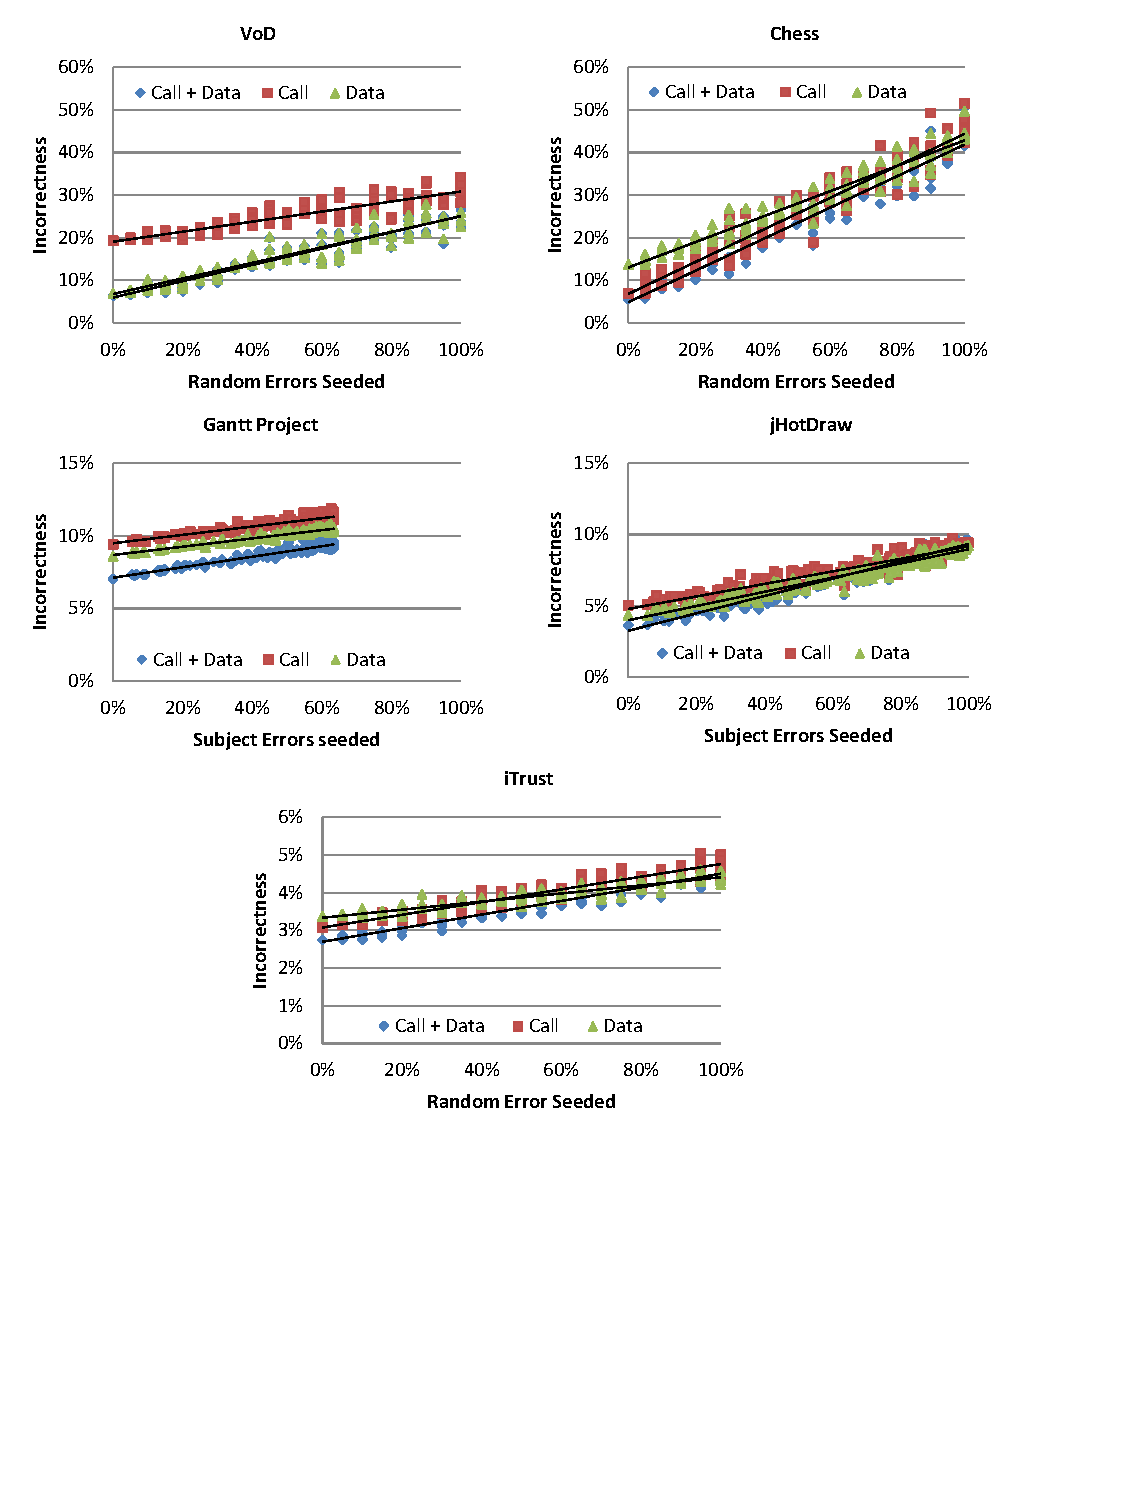
\includegraphics[width=5in]{figure/chapter4/errorExpCH4.pdf}
  \caption{以含错误的RTM为输入的五个系统上三个实验(Call,Data,Call+Data)的错误率(Incorrectness)}\label{fig_errorExpCH4}
\end{figure}

\textbf{注意:不要删除项目下面的njulogo、njuname和reviewPlaceholder这三个文件,分别是论文封面的校徽、手写体南大校名以及盲审时的空白占位符。}

\section{引用代码}

\begin{figure}[htb]
  \centering
  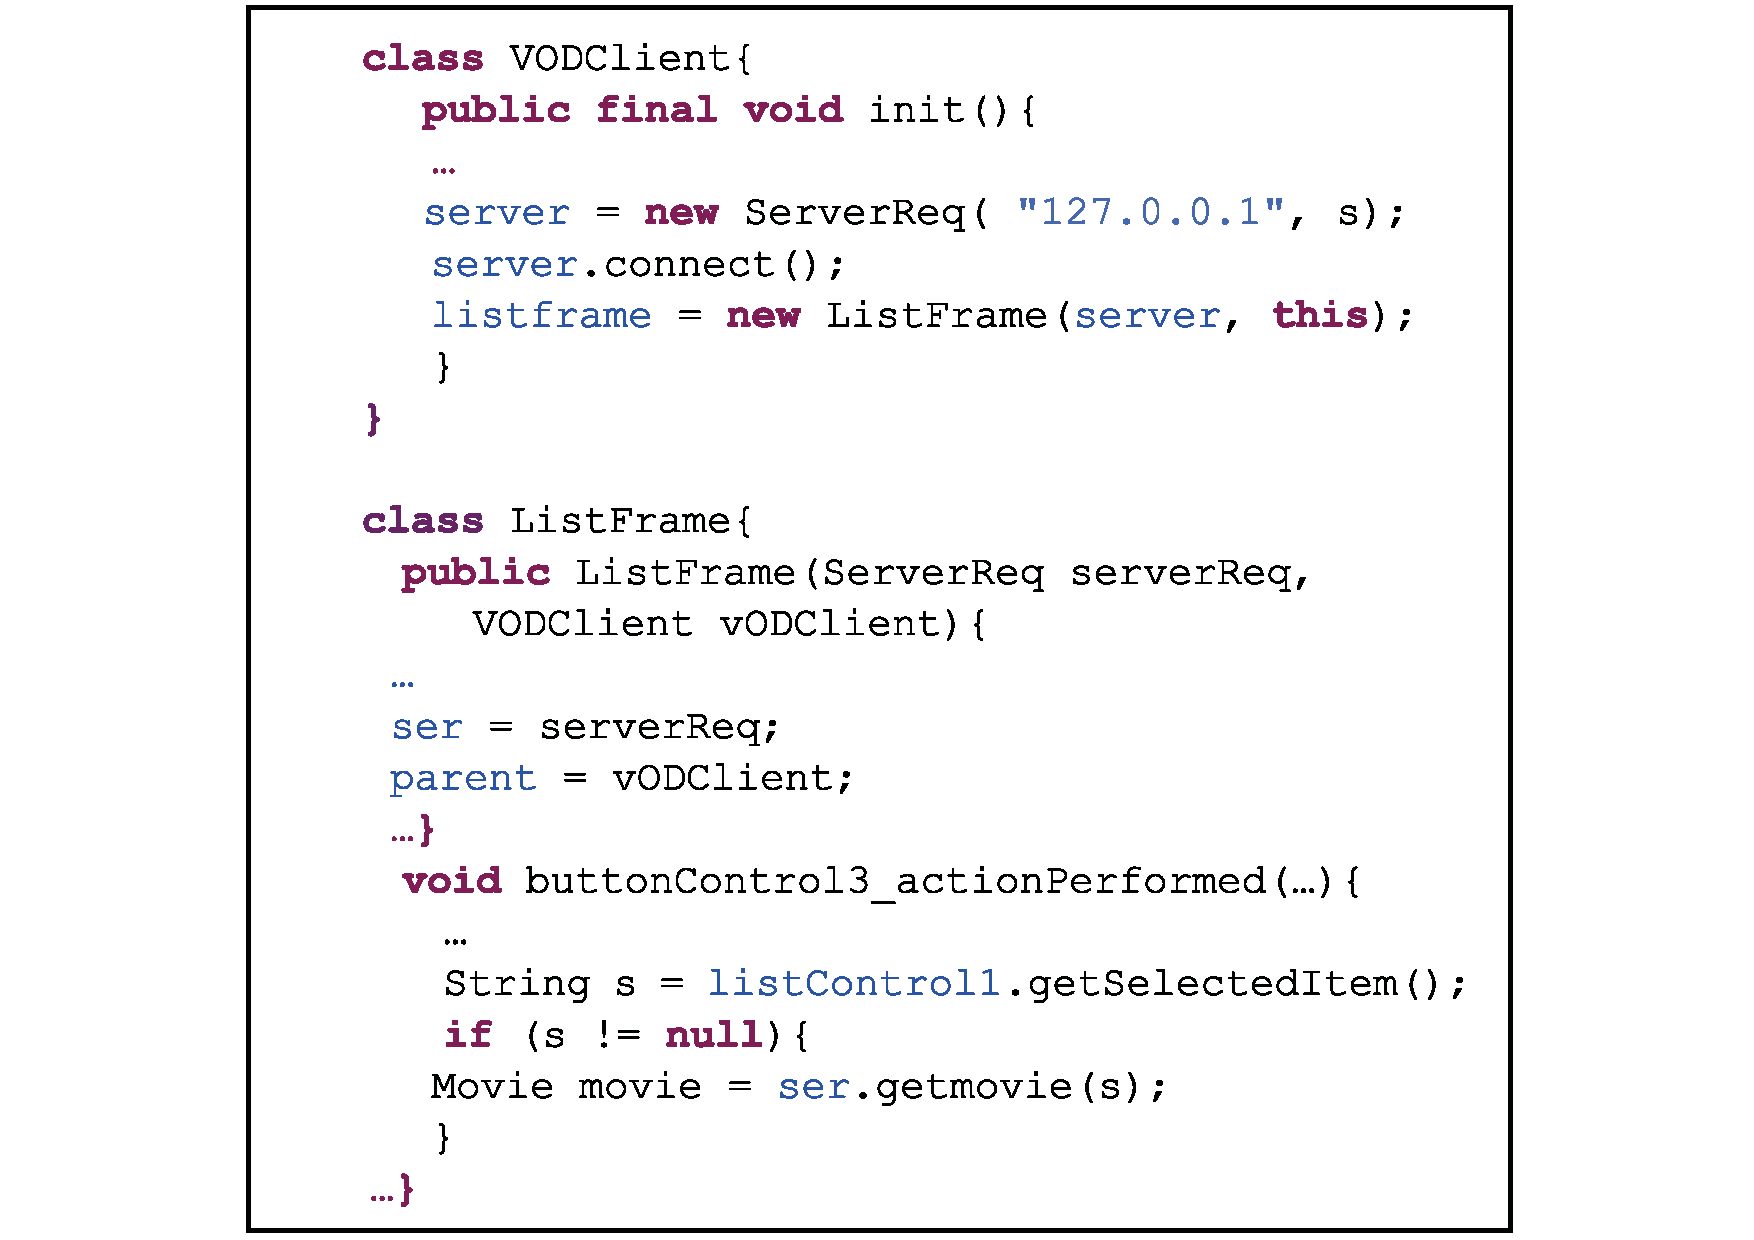
\includegraphics[width=\linewidth]{figure/chapter4/VoDCodeSample.pdf}
  \caption{VoD系统中的代码片段}\label{fig_VoDCodeSample}
\end{figure}

这里给出一个代码引用的推荐实践。
引用代码时先将代码放入word的文本框中,调整结束后,将该文本框页面另存为pdf文件,之后再作为图形来引用,如图~\ref{fig_VoDCodeSample}所示。

\section{其它图引用}

这里给出原模板提供的插图例子,请注意多行多图的设置方式。

一行一图,如图\ref{fig:line}。
\begin{figure}[htbp]
	\centering
	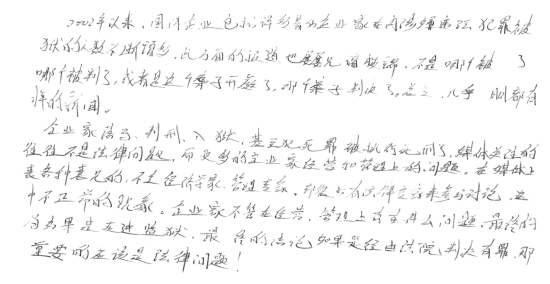
\includegraphics[width=0.7\textwidth]{figure/line.png} % requires the graphicx package
	\caption{待分行文本}
	\label{fig:line}
	%\vspace{0.8cm} % 用来调整和下方文字的间距
\end{figure}


一行两个图,如图\ref{fig:lstm}。
\begin{figure}[ht!]
	\centering
	\begin{subfigure}{.5\textwidth}
		\centering
		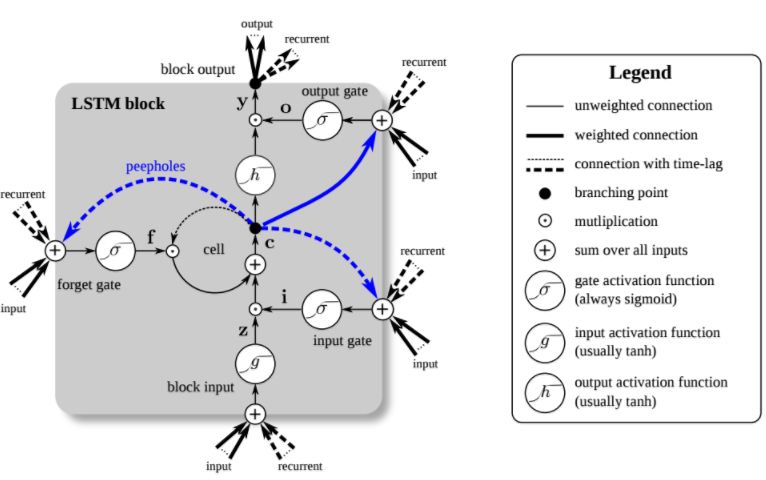
\includegraphics[width=0.9\textwidth]{figure/lstm1.png}
		\caption{长短时记忆单元模块}
	\end{subfigure}
	\begin{subfigure}{.4\textwidth}
		\centering
		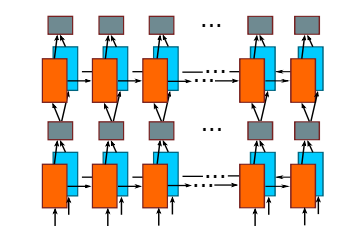
\includegraphics[width=0.8\textwidth]{figure/lstm2.png}
		\caption{深双向长短时记忆}
		\label{fig:lstm2}
	\end{subfigure}
	\caption{(a)一个长短时记忆单元模块。(b)深度双向长短时记忆的结构。}
	\label{fig:lstm}
\end{figure}

多行多图,如图\ref{fig:multi}。注意源文件中的双空行起到了子图换行的作用。
子图中大小不一是有意为之,请留意源码中subfigure和includegraphics后面的命令与四个子图大小之间的关系。

\textbf{注意:后续连续出现图形是最终文档中需要避免的情况,一般而言出现这种情况都是图贴的太多,文字写的太少导致的。建议针对每个图或表都采用“三段论”,即给出图表之前先介绍图表的大致情况与理由,然后给出图表,在图表展示之后再对图表中的内容进行讨论。}

\begin{figure}[ht!]
	\centering
	\begin{subfigure}{.69\textwidth}
		\centering
		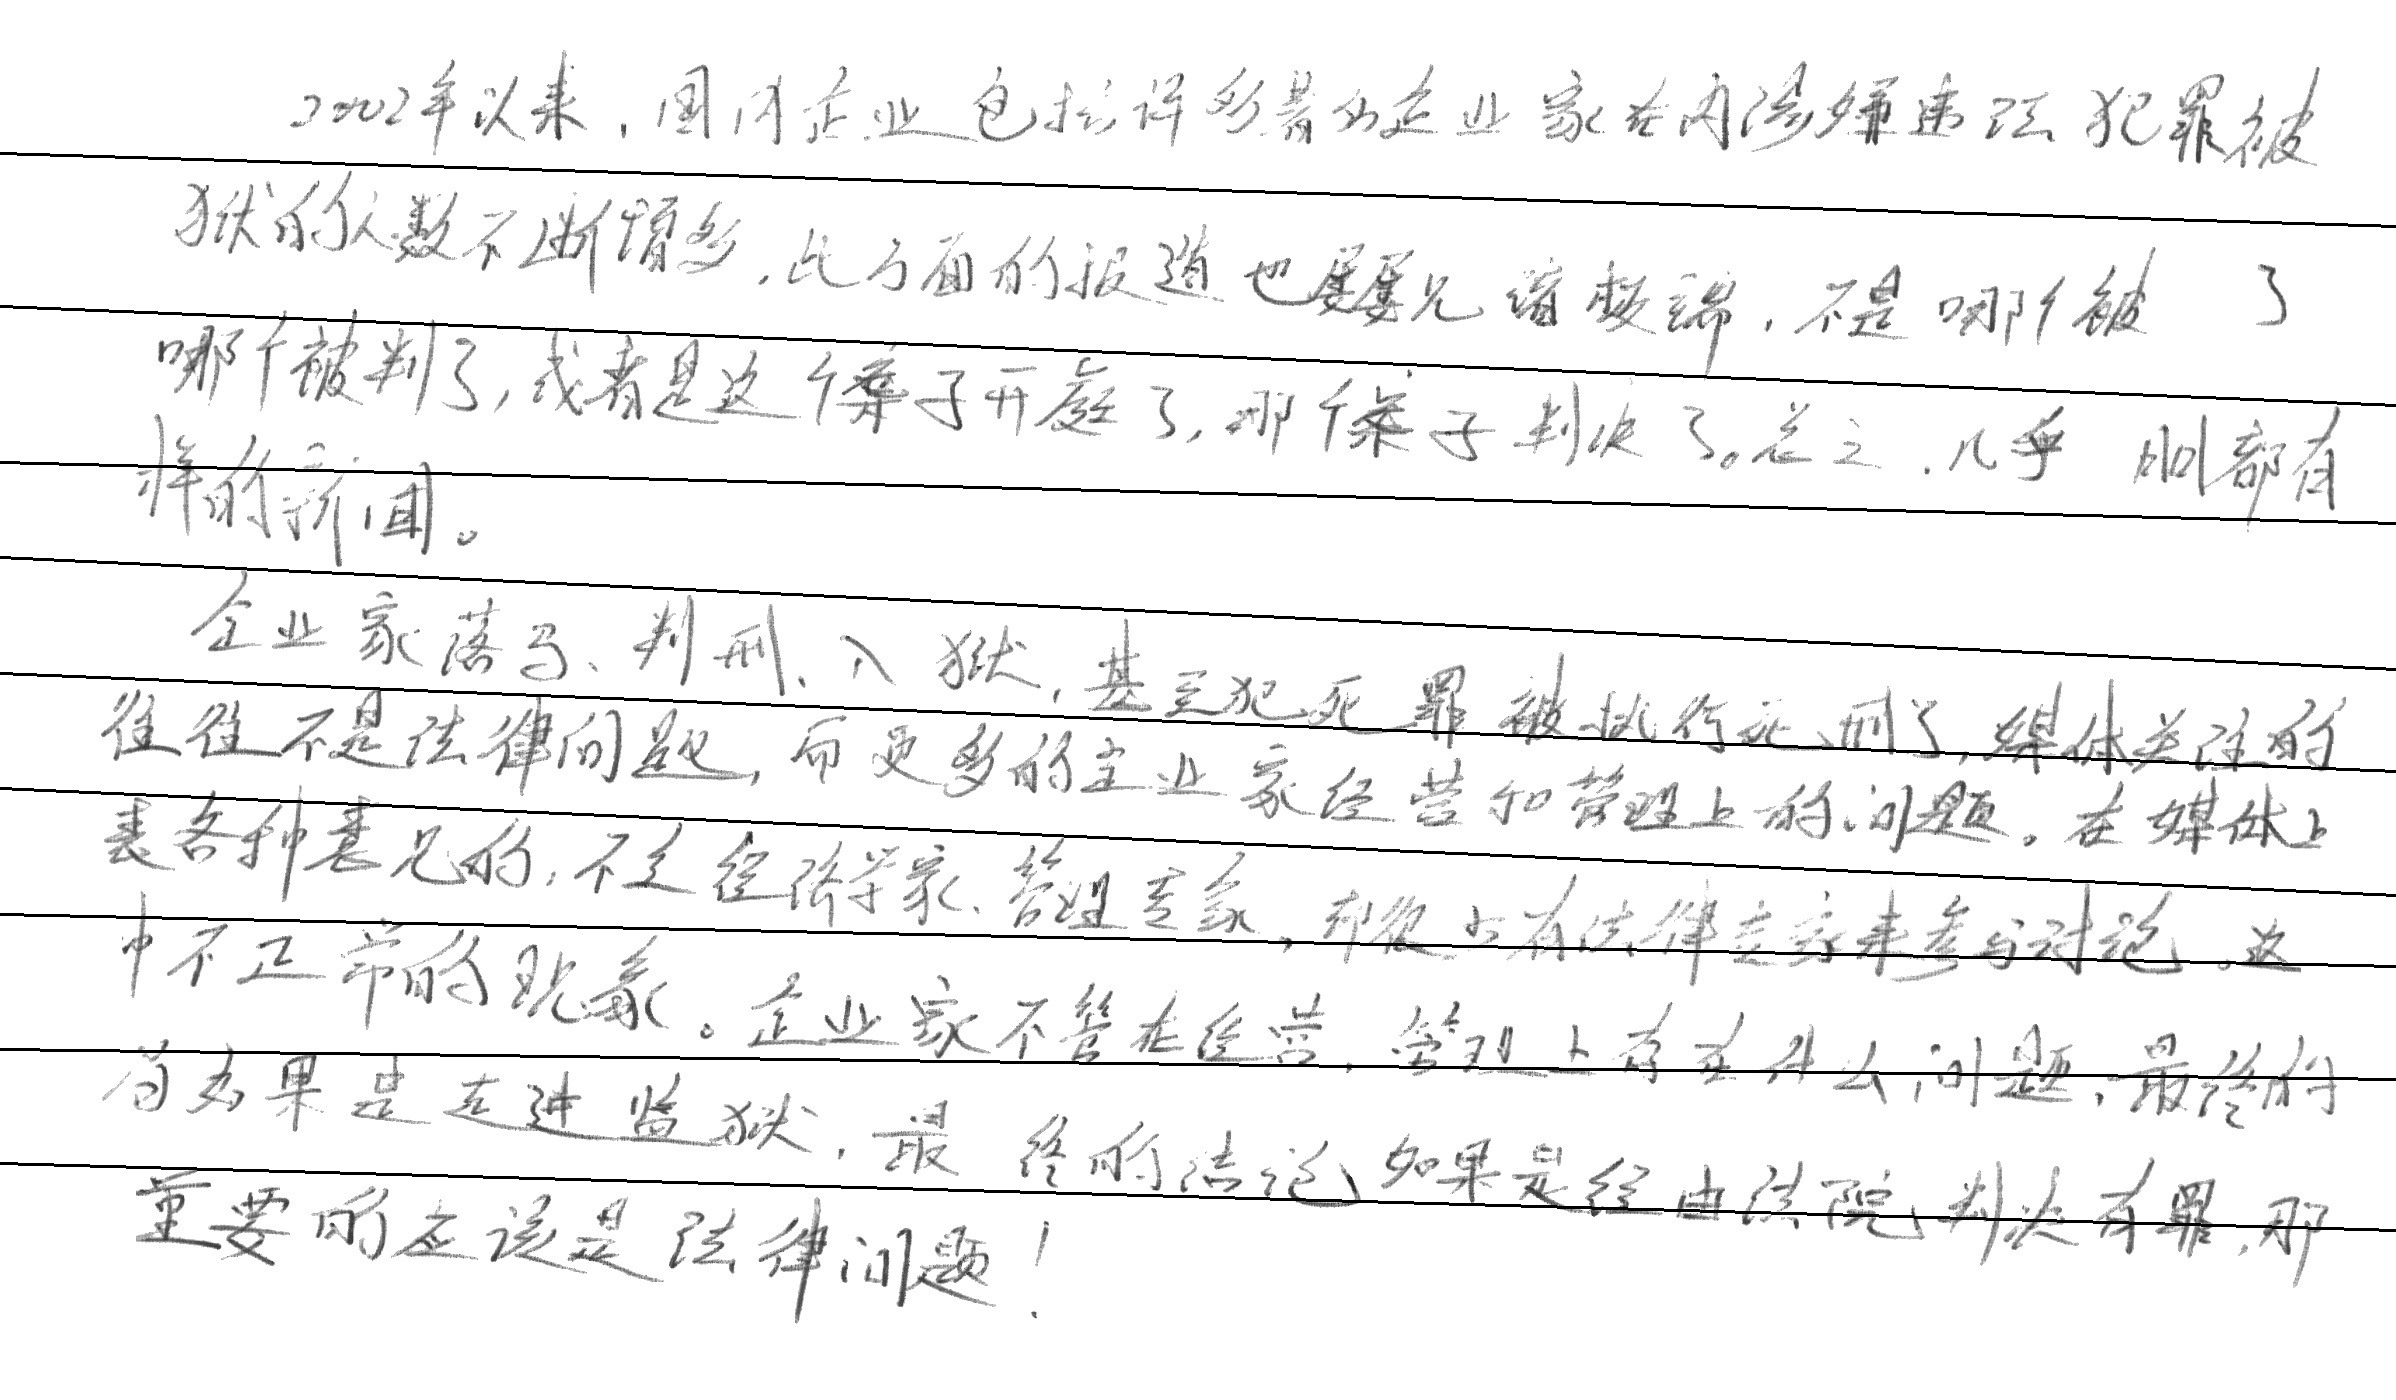
\includegraphics[width=1.0\textwidth]{figure/line1.png}
		\caption{全局损失切割第一行}
		\label{fig:line1}
	\end{subfigure}
	\begin{subfigure}{.3\textwidth}
		\centering
		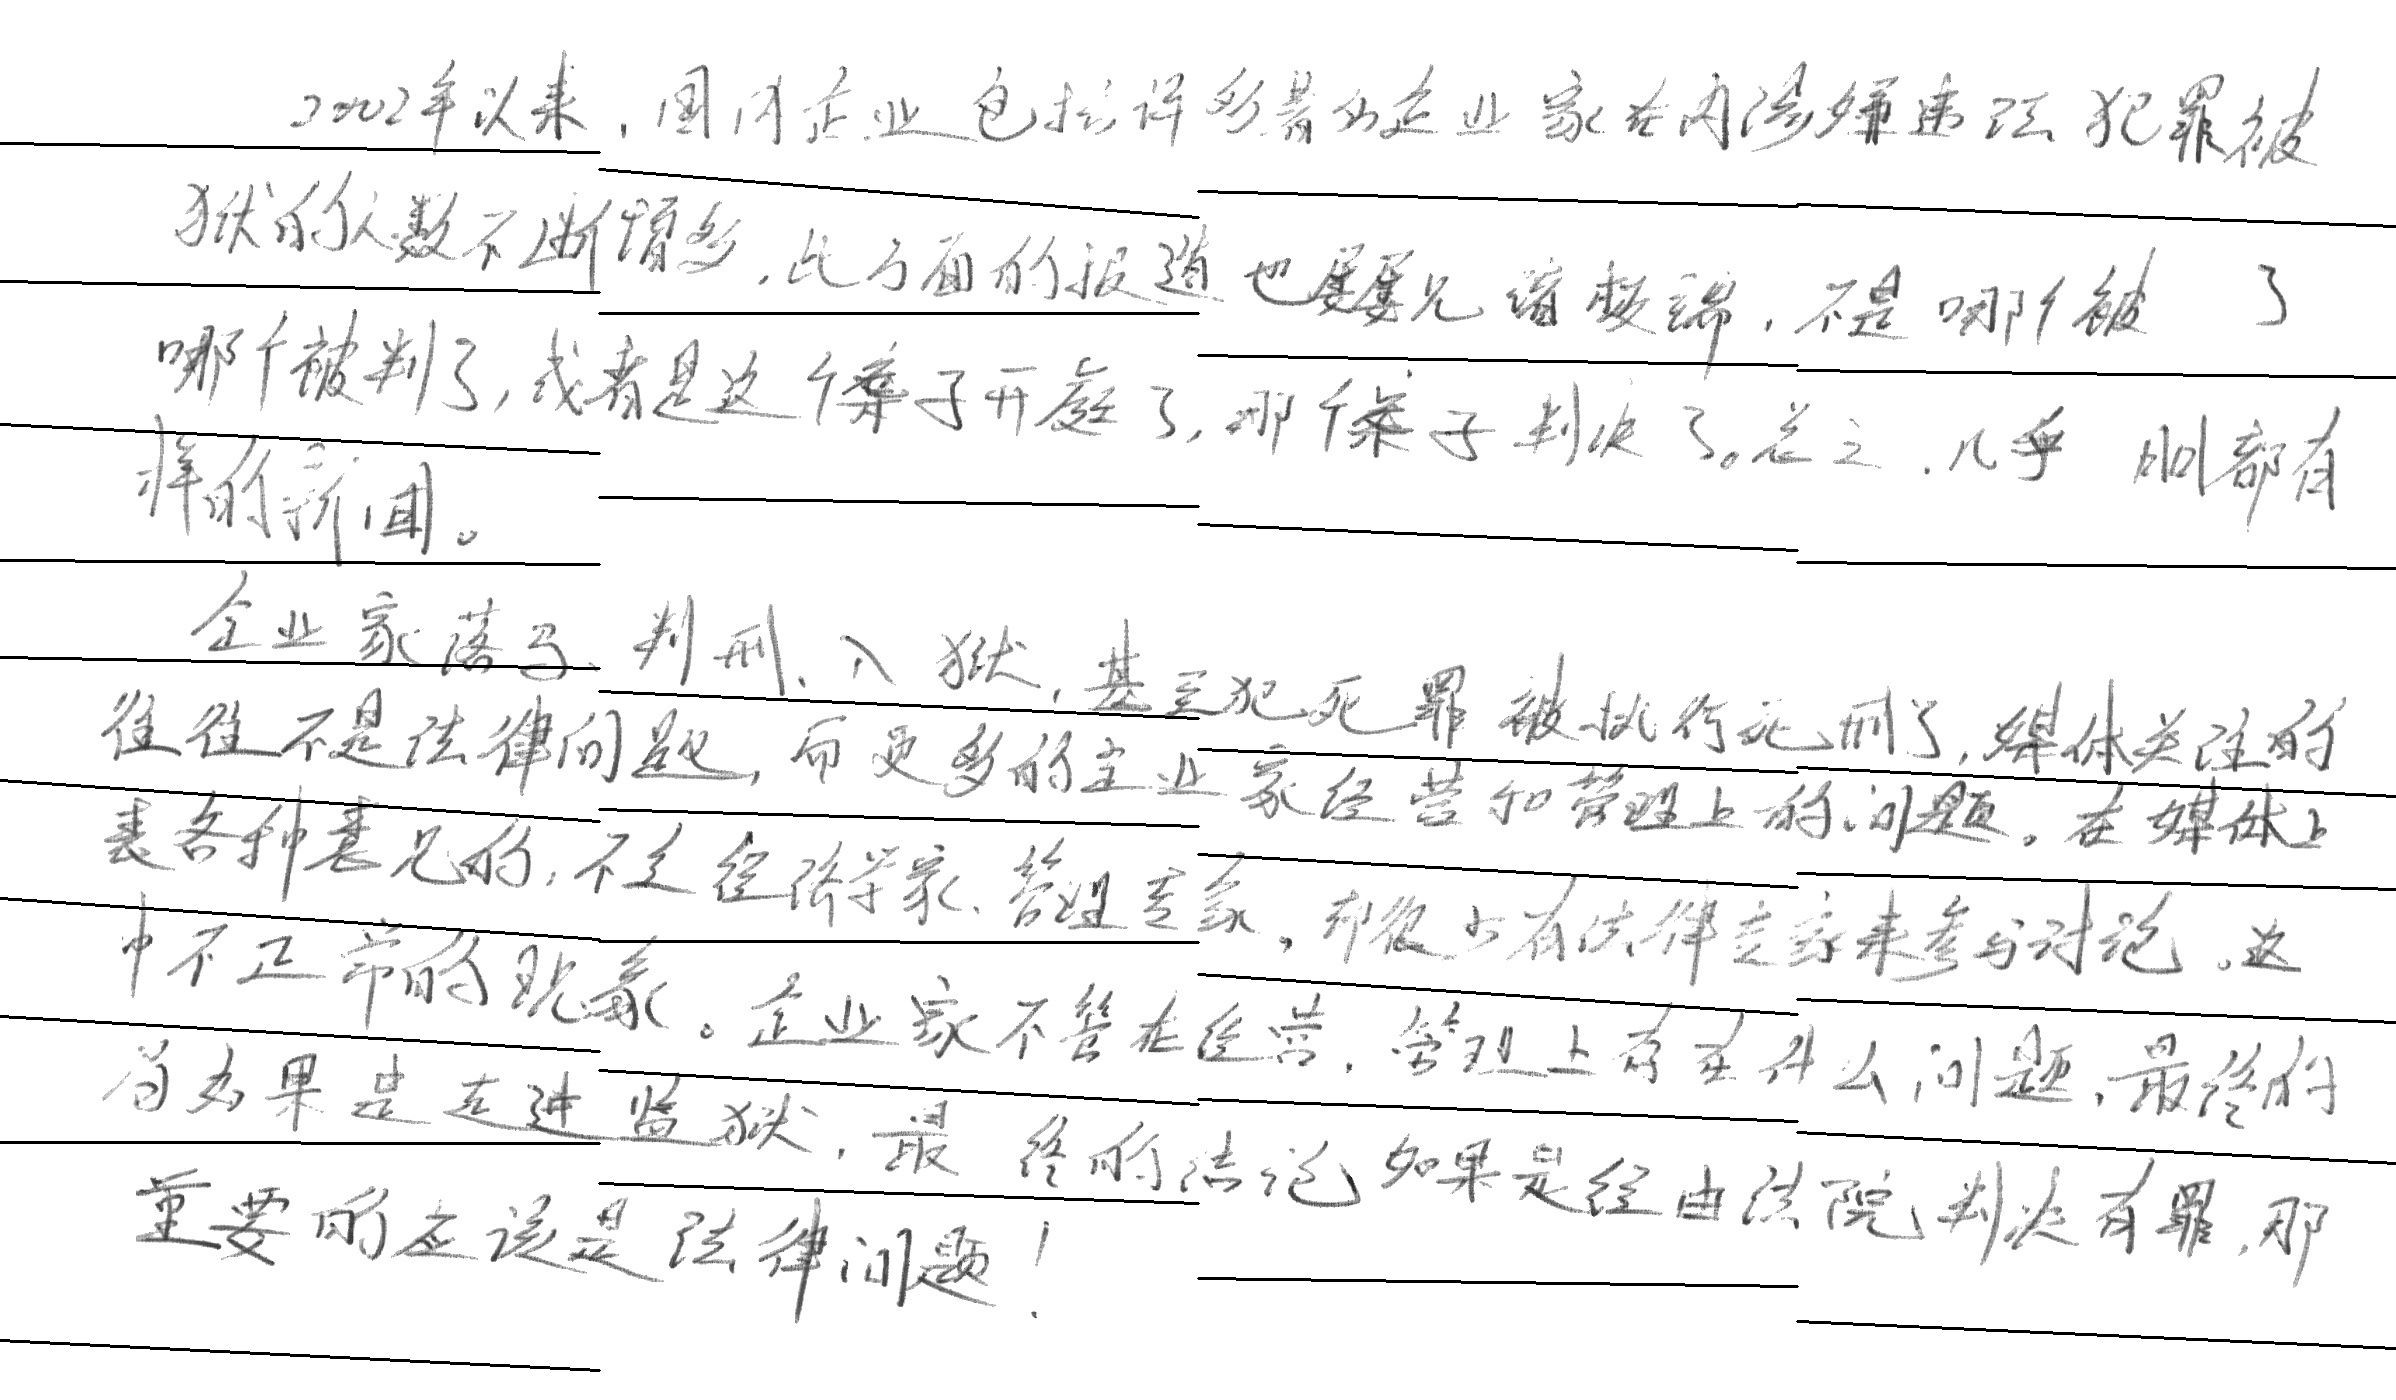
\includegraphics[width=1.0\textwidth]{figure/line2.png}
		\caption{局部损失切割第一行}
		\label{fig:line2}
	\end{subfigure}
	
	
	\begin{subfigure}{.49\textwidth}
		\centering
		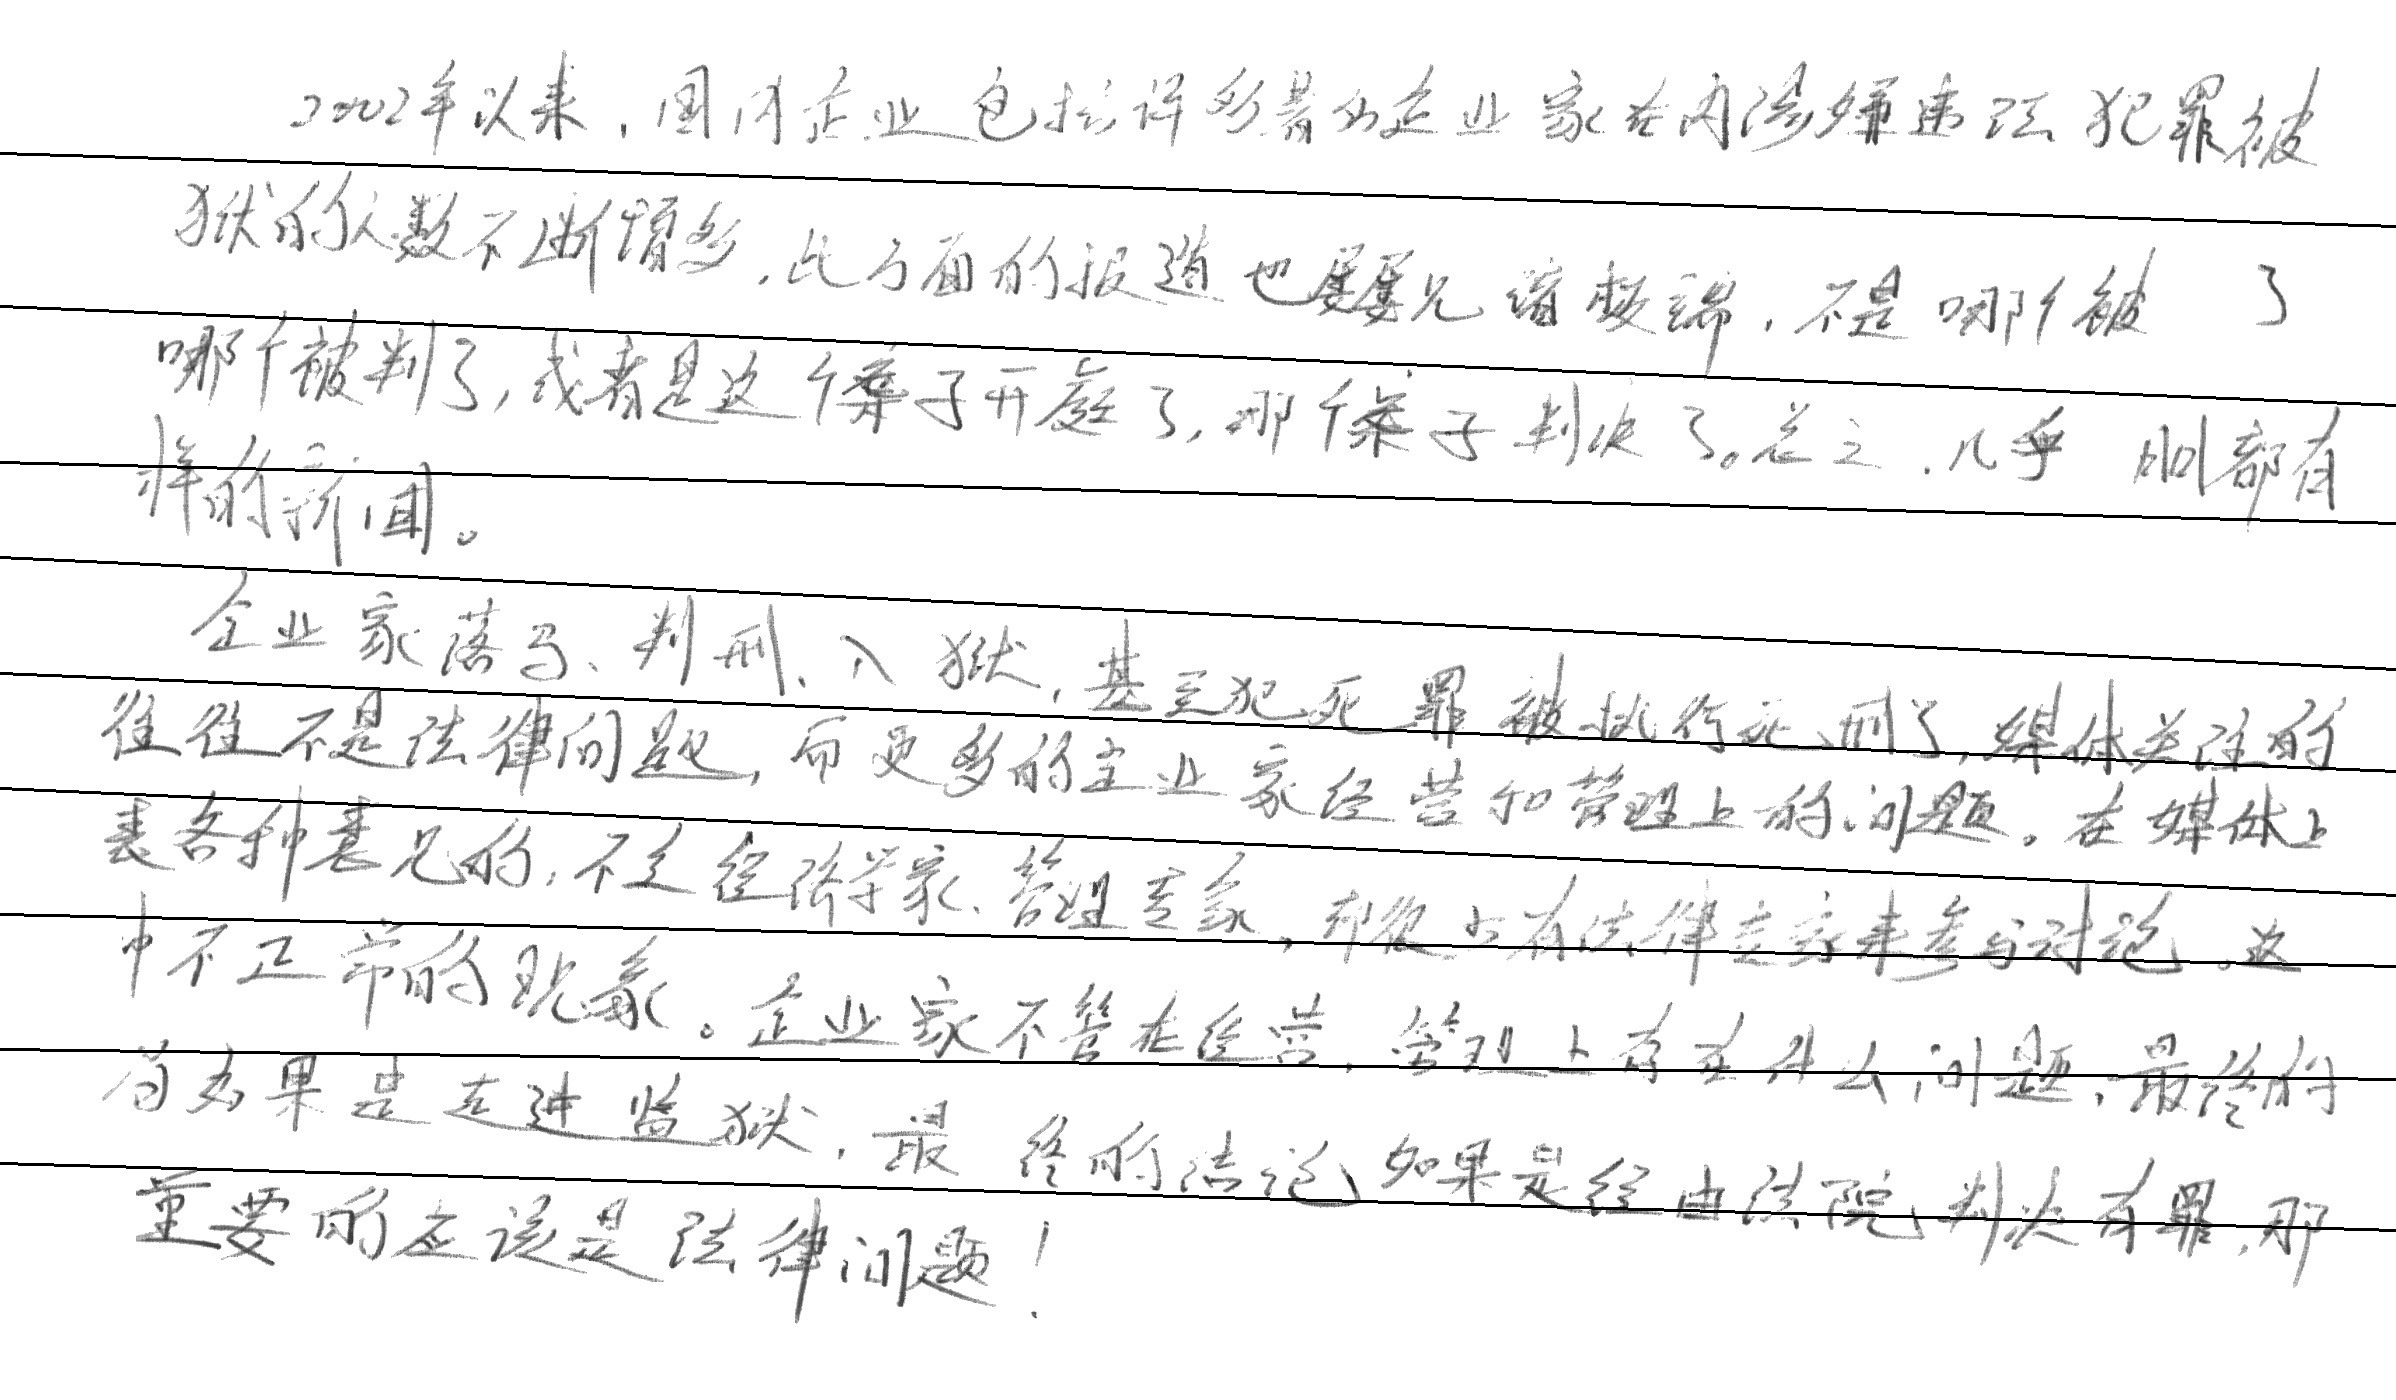
\includegraphics[width=0.5\textwidth]{figure/line1.png}
		\caption{全局损失切割第二行}
		\label{fig:line1}
	\end{subfigure}
	\begin{subfigure}{.49\textwidth}
		\centering
		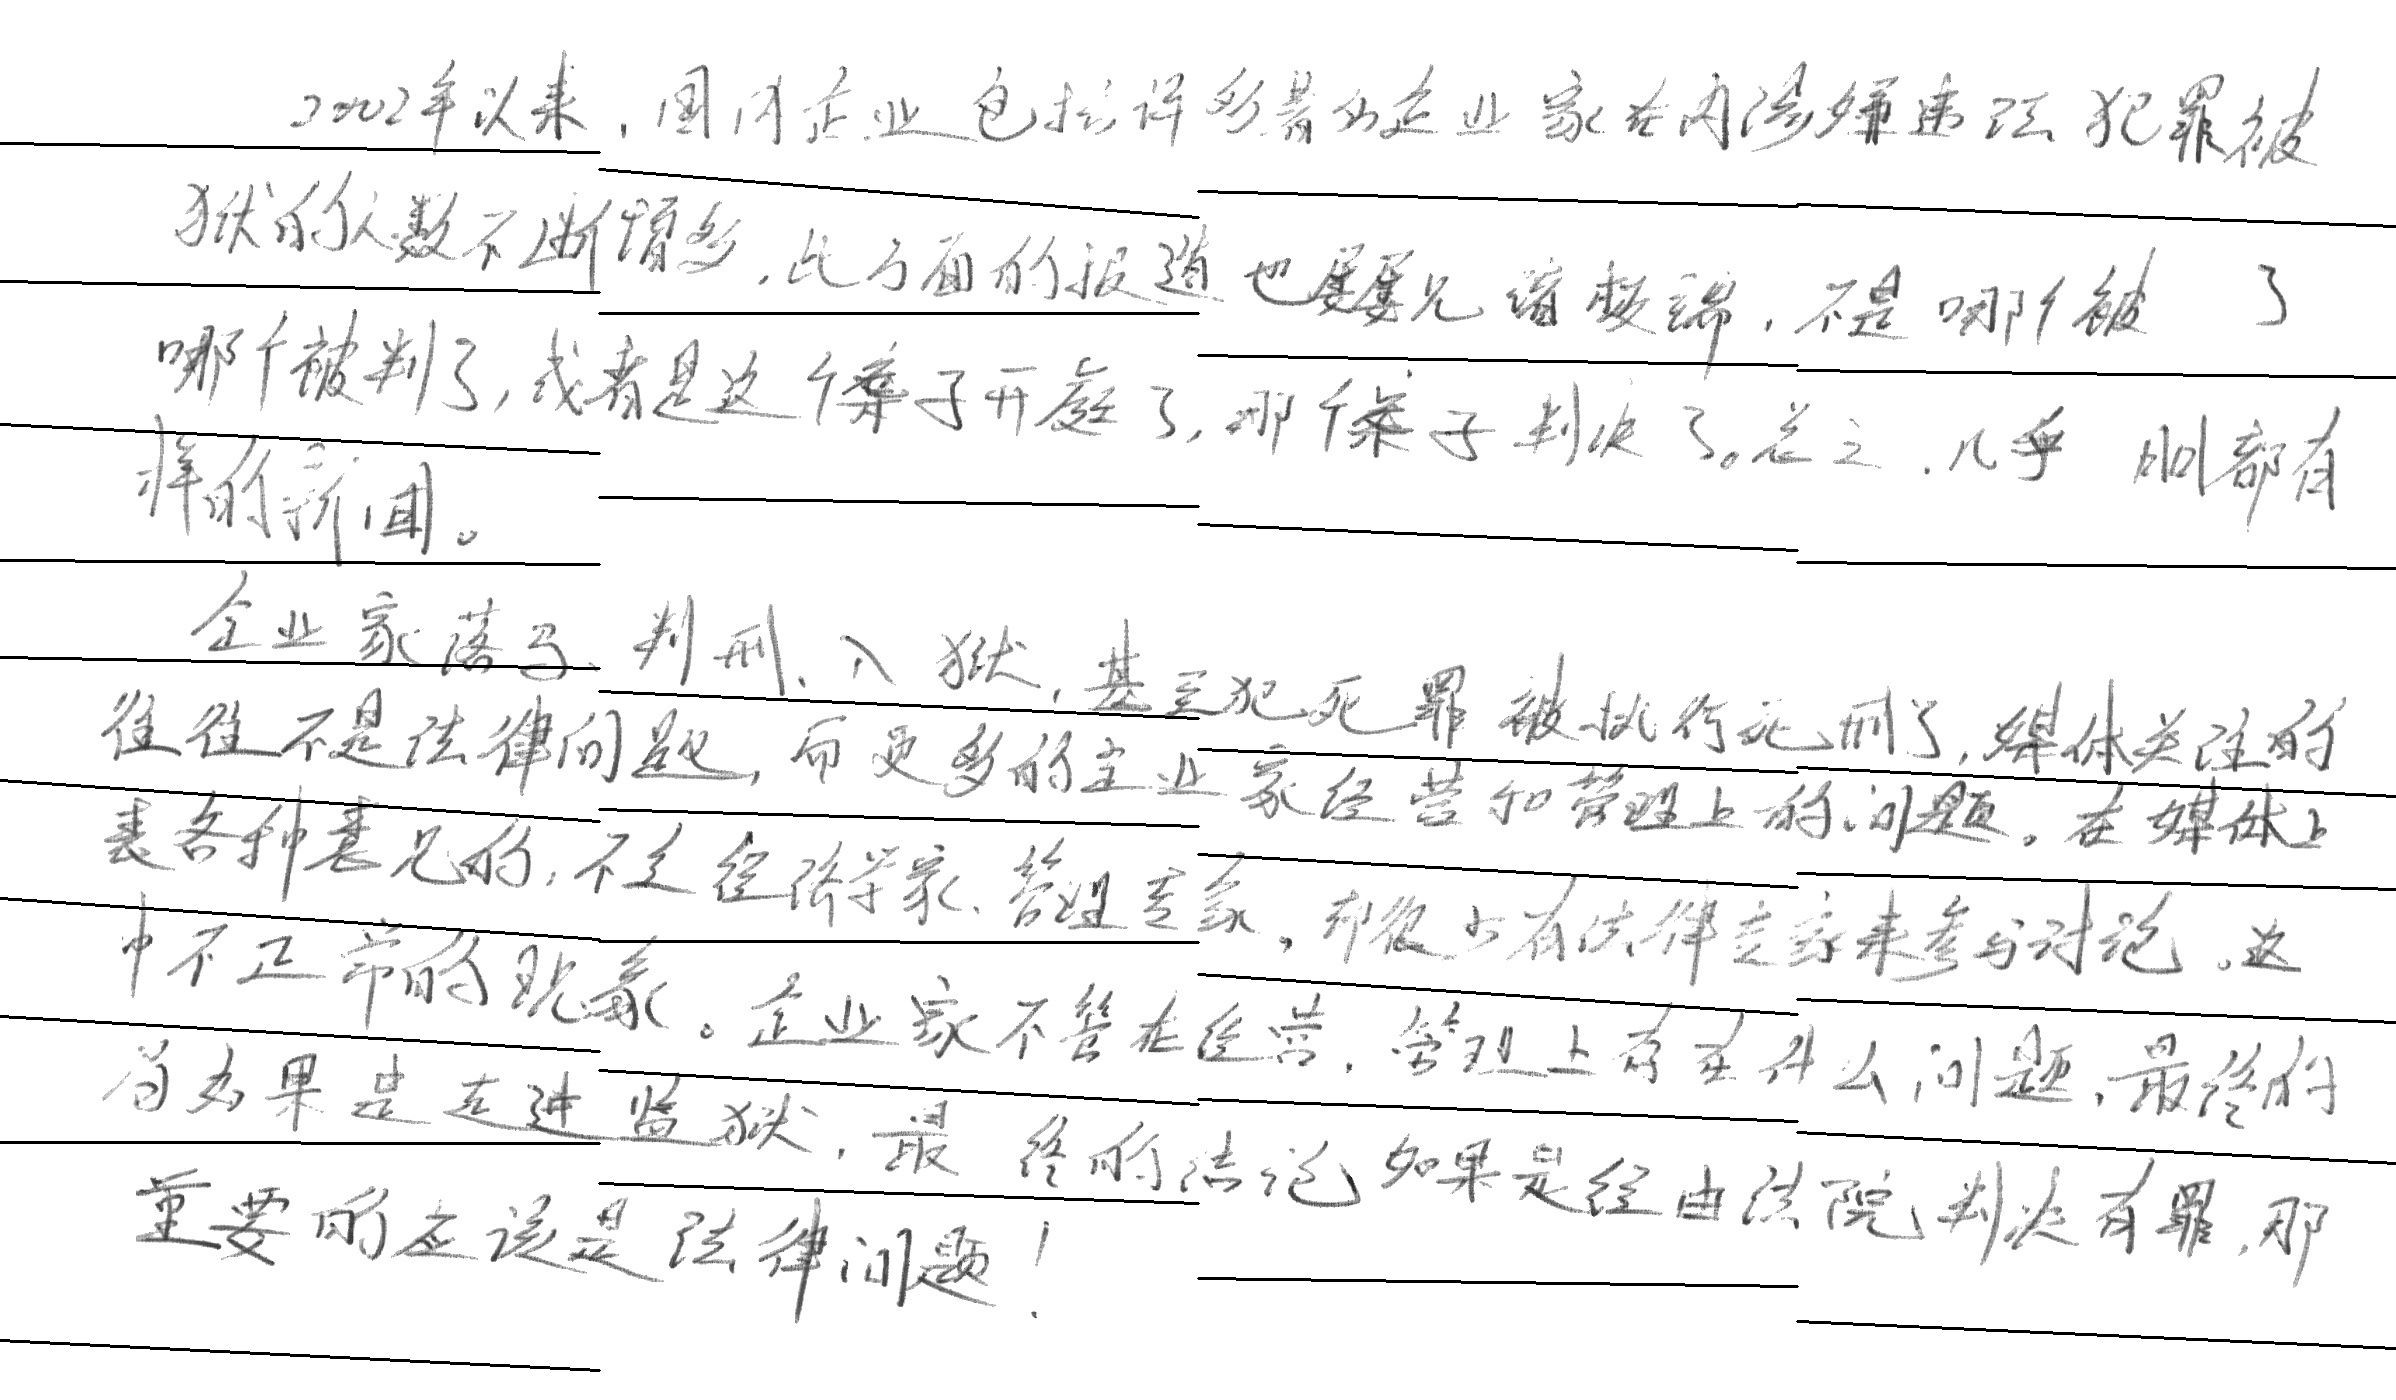
\includegraphics[width=0.8\textwidth]{figure/line2.png}
		\caption{局部损失切割第二行}
		\label{fig:line2}
	\end{subfigure}
	\caption{分行结果比较。(a)全局损失切割;(b)局部损失切割;(c)缩放的全局损失切割;(d)缩放的局部损失切割}
	\label{fig:multi}
\end{figure}

\newpage %为了将图片实例放在一起,另起一页,使用时请删掉




\chapter{公式}

这里直接给出几个较为复杂的公式的例子,可一一进行参照。
若有未包含的数学符号或公式格式,请参阅本模板所包含的手册(本地manual文件夹)或百度必应谷歌。
介绍公式时不妨也采用下面的方式,即先介绍公式的目的,给出公式,并逐一介绍公式中的变量。

\section{公式5.1与论证}
“从直接代码依赖的角度出发,从一个初始域外的类$C_{out}$ 出发我们尝试找到一个通往初始域内的类$C_{in}$ 的路径。一条合法的路径需要满足以下两点要求:(1)这一路径是单向的,即$C_{out}$ 传递性地到达$C_{in}$ 或$C_{in}$ 传递性地到达$C_{out}$;(2)路径中只能包含一个$C_{in}$ (为了避免重复路径的出现)。为了恰当的估计一条合法路径所代表的交互程度,我们计算路径上所有直接代码依赖的紧密度值的几何平均。我们用如下公式来重新计算给定$C_{out}$ 的IR 值($IR_{DC}$):”

\begin{align}
IR_{DC}=IR_{origin}+(IR_{top}-IR_{origin})^{\left| PATH\right|}\sqrt {\prod _{x \in PATH}Closeness_{DC}(x)} \end{align}

“其中$IR_{origin}$ 代表$C_{out}$ 的初始IR值,$IR_{top}$ 代表$C_{in}$ 被提升过的IR值,\emph{PATH} 代表$C_{out}$ 与$C_{in}$ 之间的路径内所有的直接代码依赖,而$Closeness_{DC}(x)$ 则代表每一条直接代码依赖关系的紧密度值。在同一对$C_{out}$ 和$C_{in}$ 之间可能存在多条合法路径,我们只保留其中能使$IR_{DC}$ 值最大的那条路径。”

\section{公式5.2与论证}

“由于IR 方法返回的是一个按照IR 值大小倒序排列的候选线索列表,因此一种常用的比较IR 方法的方式是在不同的查全率水平上比较不同方法之间的精确度,通常用$Precision-Recall$ 曲线表示。为了进一步衡量IR 方法返回结果的整体质量,我们选用了另外两个常用的实验度量:$AP$(Average Precision)与$MAP$ (Mean Average Precision)。其中,$AP$ 用于度量全部查询(需求)所检索的相关文档的排序质量,计算方式如下:”
\begin{align}
AP=\dfrac {\sum _{r=1}^{N}\left( Precision\left( r\right) \times isRelevant\left( r\right) \right) } {\left| RelevantDocuments\right| }
\end{align}

“其中,$r$ 表示被查询对象(类)在列表中的排序,$Precision(r)$ 表示前$r$ 个类的准确率。$isRelevant()$ 为一个二值函数,如果文档是相关的,则返回1,若无关,则返回0。”

\section{公式5.3与论证}

“由此,我们为类数据依赖定义紧密度$Closeness_{CD}$ 如下:”

\begin{align}Closeness_{CD}=\frac {\sum _{x \in \{DT_{i}\cap DT_{j}\}}idtf(x)} {\sum _{y \in \{DT_{i}\cup DT_{j}\}}idtf(y)}\end{align}

“其中$idtf(x)$ 代表共享数据类型的idtf值,$DT_i$ 与$DT_j$ 的交集代表该数据依赖上的共享数据类型,而$DT_i$ 与$DT_j$ 的并集则代表$C_i$ 和$C_j$ 在全部代码上所访问的数据类型。$Closeness_{CD}$ 的取值范围是0到1之间。”

\section{原模板中的其它公式}

\begin{equation}
\frac{\partial L}{\partial a_{k}^t} = {d(s)}^2 (y_{k}^t - \frac{\sum_{lab(\mathbf{l},k)} \alpha_t(s)\beta_t(s) }{y_{k}^t} )
\end{equation}

\begin{equation}
\begin{aligned}
d_{{0j}}&=\sum _{{k=1}}^{{j}}w_{{\mathrm  {ins}}}(a_{{k}}),\quad &{\text{for}}\;1\leq j\leq n\\
d_{{ij}}&={\begin{cases}d_{{i-1,j-1}}&{\text{for}}\;a_{{j}}=b_{{i}}\\\min {\begin{cases}d_{{i-1,j}}+w_{{\mathrm  {del}}}(b_{{i}})\\d_{{i,j-1}}+w_{{\mathrm  {ins}}}(a_{{j}})\\d_{{i-1,j-1}}+w_{{\mathrm  {sub}}}(a_{{j}},b_{{i}})\end{cases}}&{\text{for}}\;a_{{j}}\neq b_{{i}}\end{cases}}\quad &{\text{for}}\;1\leq i\leq m,1\leq j\leq n.
\end{aligned}
\end{equation}

\begin{equation}
\begin{aligned}
&\beta_T(|l{}'|)=y_{b}^{T}\\
&\beta_T(|l{}'|-1)=y_{l_|l|}^{T} \\
&\beta_T(s)=0, \forall s < |l{}'|-1
\end{aligned}
\end{equation}

递归公式举例(出现了公式过长的问题,实践中最好适当控制长度,给公式编号在同一行上留下位置)。
\begin{equation}
\beta_t(s)=\left\{
\begin{aligned}
& (\beta_{t+1}(s) d(s)+\beta_{t+1}(s+1))d(s+1)\,  y_{\l_s{}'}^t, \: \: if \:  l_s{}'=b \:  or \:  l_{s+2}{}'=l_s{}'\\
& (\beta_{t+1}(s) d(s)+\beta_{t+1}(s+1)d(s+1)+\beta_{t+1}(s+2)d(s+2))\,  y_{\l_s{}'}^t,\: \:   otherwise
\end{aligned}
\right.
\end{equation}


\chapter{算法}

同样是定义加上引用的方式,参见算法~\ref{alg:beam}。
本算法已包含循环与分支,如有未包含的数学符号或格式,请参阅本模板所包含的手册或询问百度必应谷歌。
如论文中无需算法则不用强加。

\begin{algorithm}
	\caption{Beam Search}
	\label{alg:beam}
	\begin{algorithmic}[1]
		\STATE {将初始节点插入到集束中。} 
		\WHILE{遍历未结束}
		\STATE {遍历集束中所有节点的后续节点。} 
		\IF{该节点是目标节点}
		\STATE {算法结束。}
		\ELSE 
		\STATE {扩展该节点,取集束宽度的节点入堆。}
		\ENDIF
		\ENDWHILE
	\end{algorithmic}
\end{algorithm}

\chapter{论文引用}

\section{引文相关}
此处的论文引用采用的是类似于IEEE的按出现位置的数字编号格式。建议将被引用的论文全名放入dblp网站(必应谷歌搜索dblp)搜索,之后进入该论文详细信息,如图~\ref{fig_dblpForBibtexCH7} 所示。

\begin{figure}[htb]
  \centering
  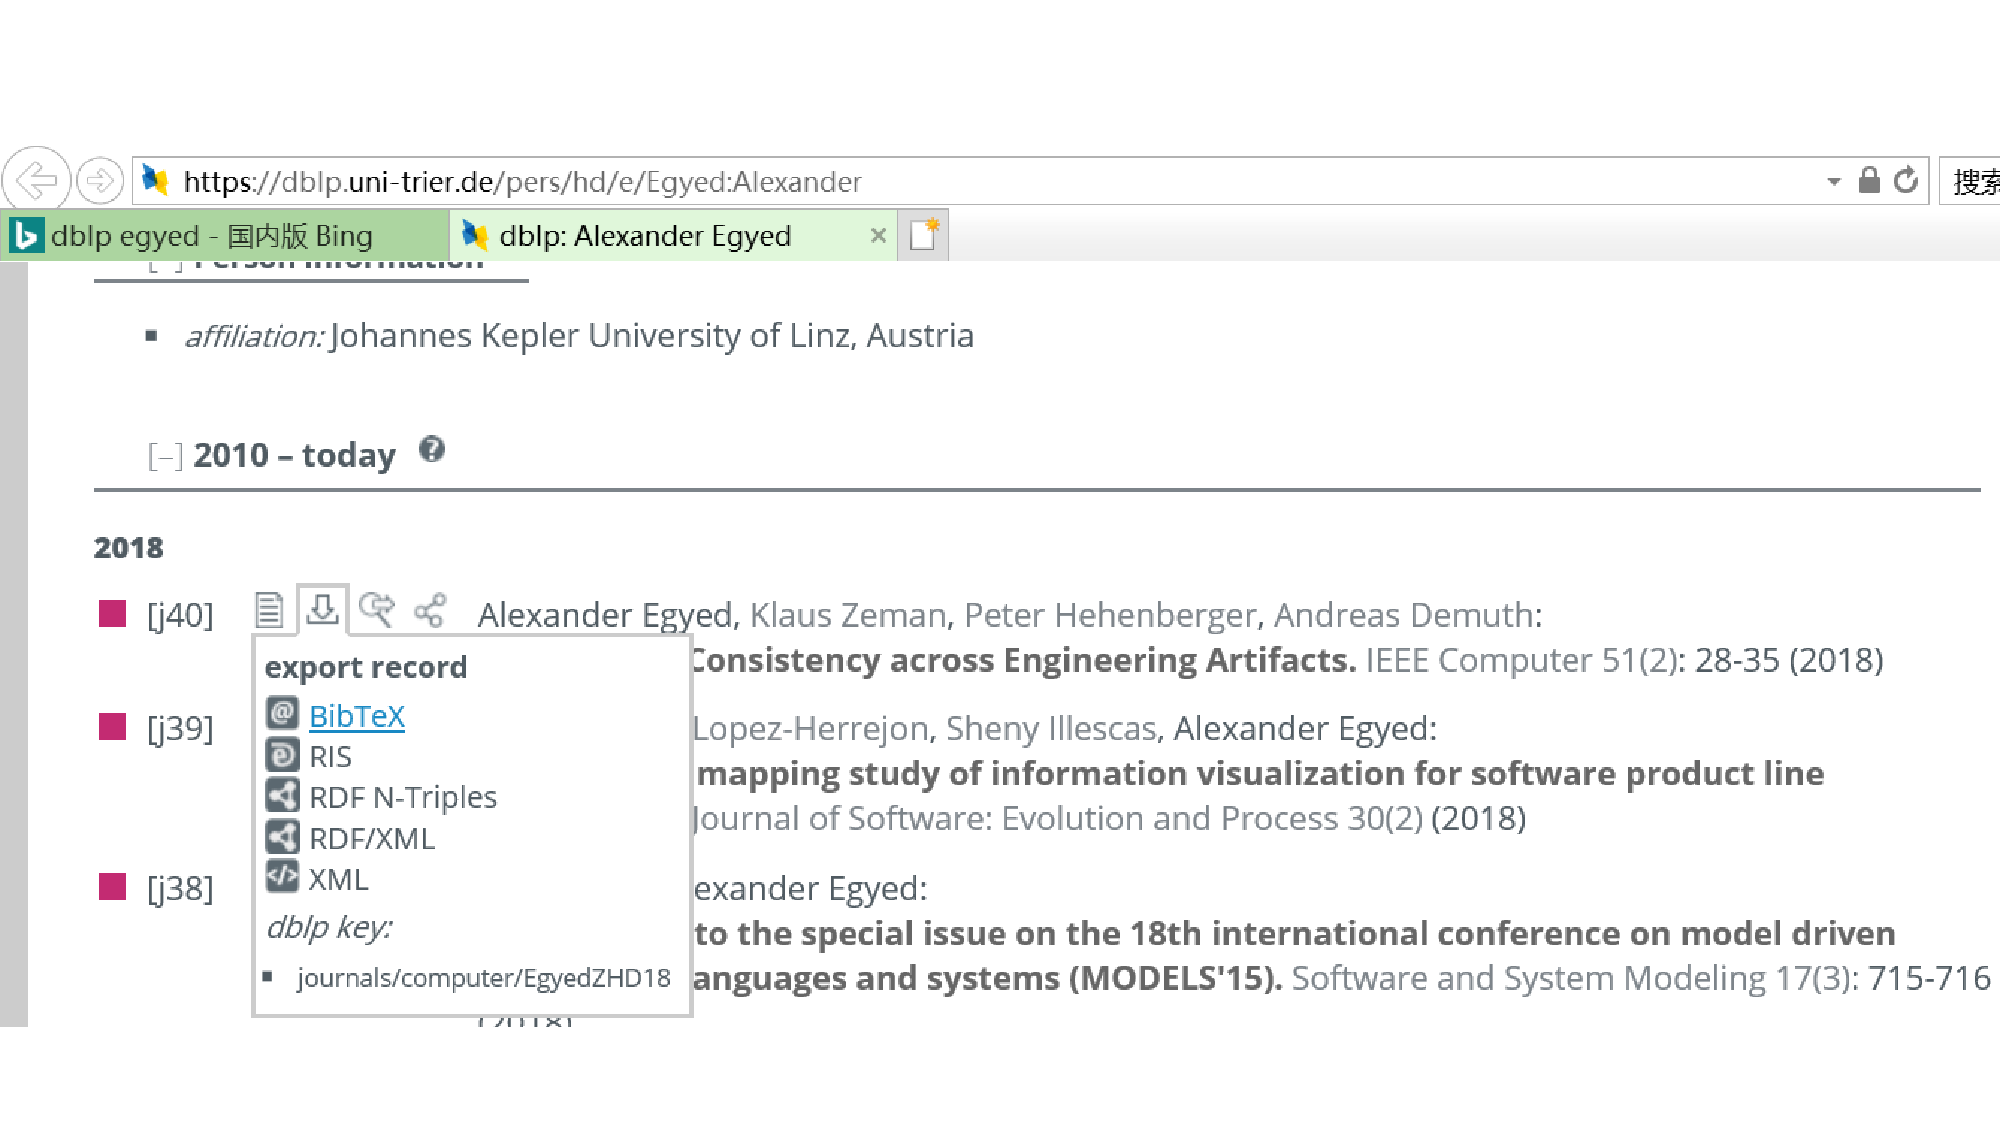
\includegraphics[width=5in]{figure/chapter7/dblpForBibtex.pdf}
  \caption{在dblp上下载Bibtex}\label{fig_dblpForBibtexCH7}
\end{figure}

点击图~\ref{fig_dblpForBibtexCH7}中所示的链接之后将得到Bibtex信息,如图~\ref{fig_bibtexDetailCH7}所示。
打开本地文件夹下的sample.bib文件,完整添加该信息。
并在需要引用的位置添加这一引用~\cite{DBLP:journals/computer/EgyedZHD18}。
格式为bibtex信息中的开头,\emph{例如图中的“DBLP:journals/computer/EgyedZHD18”。(此处是一个典型的因为长字符串导致的bad box,请参考上述章节的内容手动进行软换行)}。

\textbf{注意:在修改并保存sample.bib文件后,先编译tex文件,再编译参考文献,之后再编译两次,此时引用位置的方括号内将出现具体的编号而不是问号,且编号对应的引文已经出现在参考文献内。本模板点击引用编号后可以跳转到对应的参考文献处。}

在bib文件中出现,但并未在论文中被引用的论文不会出现在最后的参考文献中。如果dblp中并未包含你需要的论文,则可以尝试谷歌或百度学术的搜索结果,一般也包含bibtex信息,但可能不完整或不规范。

引用网站链接可以考虑这一格式~\cite{GanttSystemWeb}(不推荐,网站链接使用脚注更规范些)。

引用书籍可以考虑这一格式~\cite{Pohl2010Requirements}。

中文文献请参考这一格式~\cite{cyg2006}(引用标记不要使用中文,否则容易出现编译错误)。

以下英文引用用来测试引文排序是否按照插入顺序,以及多引文是否合并~\cite{DBLP:journals/computer/EgyedZHD18, DBLP:journals/ml/TingZCZWZ19}

\begin{figure}[htb]
  \centering
  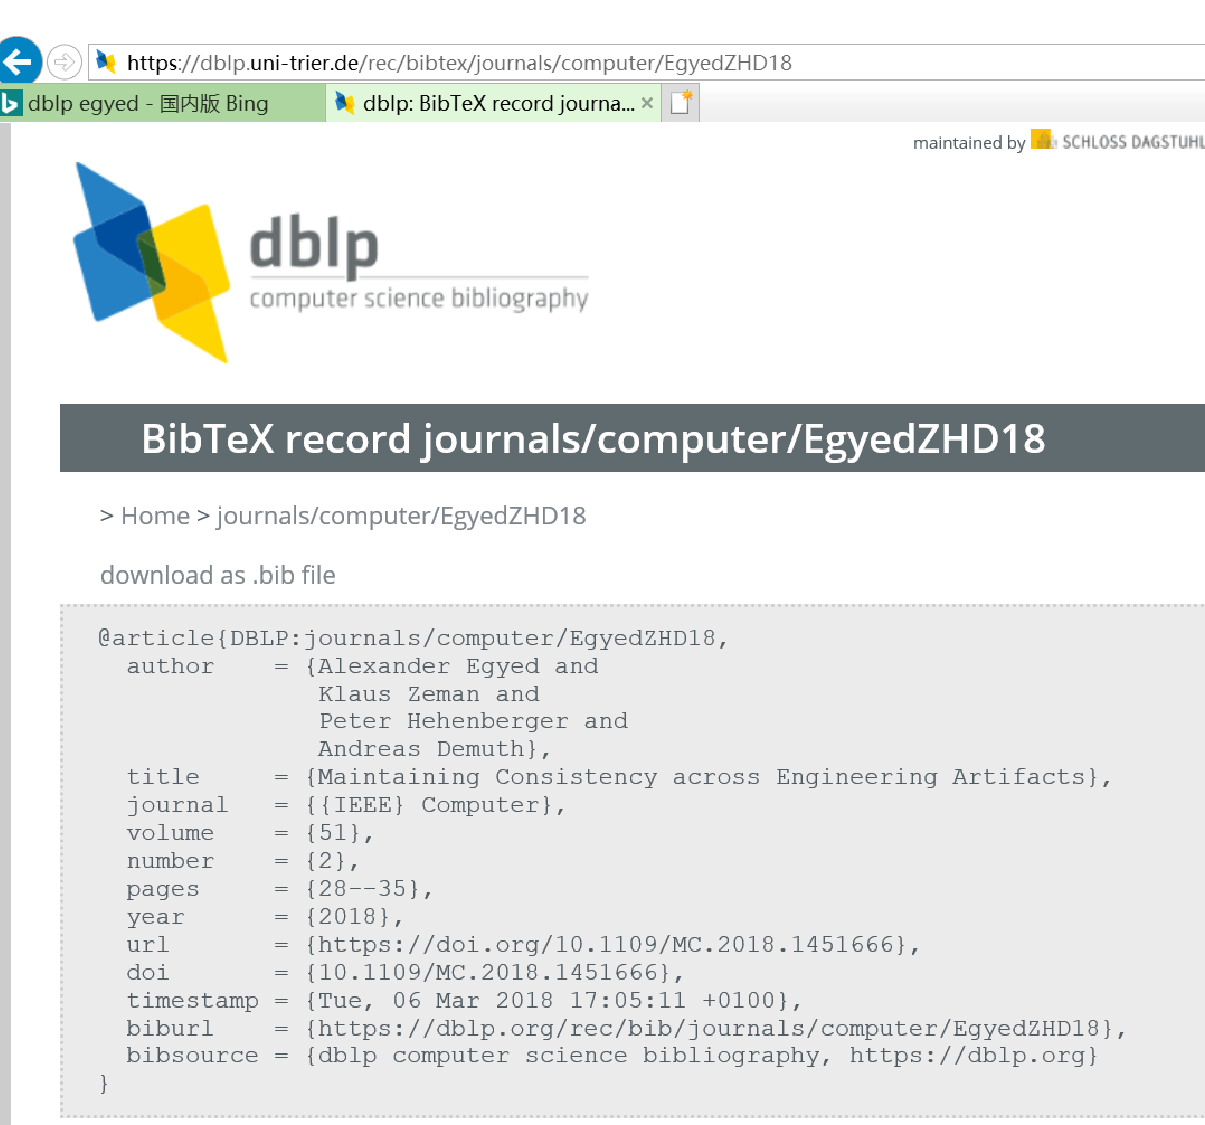
\includegraphics[width=5in]{figure/chapter7/bibtexDetail.pdf}
  \caption{Bibtex详细信息}\label{fig_bibtexDetailCH7}
\end{figure}


%%%%%%%%%%%%%%%%%%%%%%%%%%%%%%%%%%%%%%%%%%%%%%%%%%%%%%%%%%%%%%%%%%%%%%%%%%%%%%%
% 致谢,应放在结论之后
\begin{acknowledgement}
	感谢在实验室度过的两年时光,老师无论在学术还是人生的指导上都对我起到了很大的帮助;师兄师姐小伙伴们的鼓励支持和陪伴是我坚持下去的动力。
\end{acknowledgement}




% 参考文献。应放在\backmatter之前。
% 推荐使用BibTeX,若不使用BibTeX时注释掉下面一句。
%\nocite{*}
\bibliography{sample}


% 附录,必须放在参考文献后,backmatter前
\appendix
\chapter{附录代码}\label{app:1}
\section{main函数}
\begin{lstlisting}[language=C]
int main()
{
	return 0;
}
\end{lstlisting}

%%%%%%%%%%%%%%%%%%%%%%%%%%%%%%%%%%%%%%%%%%%%%%%%%%%%%%%%%%%%%%%%%%%%%%%%%%%%%%%
% 书籍附件
\backmatter
%%%%%%%%%%%%%%%%%%%%%%%%%%%%%%%%%%%%%%%%%%%%%%%%%%%%%%%%%%%%%%%%%%%%%%%%%%%%%%%
% 作者简历与科研成果页,应放在backmatter之后
\begin{resume}
% 论文作者身份简介,一句话即可。
\begin{authorinfo}
\noindent 韦小宝,男,汉族,1985年11月出生,江苏省扬州人。
\end{authorinfo}
% 论文作者教育经历列表,按日期从近到远排列,不包括将要申请的学位。
\begin{education}
\item[2007年9月 --- 2010年6月] 南京大学计算机科学与技术系 \hfill 硕士
\item[2003年9月 --- 2007年6月] 南京大学计算机科学与技术系 \hfill 本科
\end{education}
% 论文作者在攻读学位期间所发表的文章的列表,按发表日期从近到远排列。
\begin{publications}
\item Xiaobao Wei, Jinnan Chen, ``Voting-on-Grid Clustering for Secure
  Localization in Wireless Sensor Networks,'' in \textsl{Proc. IEEE International
    Conference on Communications (ICC) 2010}, May. 2010.
\item Xiaobao Wei, Shiba Mao, Jinnan Chen, ``Protecting Source Location Privacy
  in Wireless Sensor Networks with Data Aggregation,'' in \textsl{Proc. 6th
    International Conference on Ubiquitous Intelligence and Computing (UIC)
    2009}, Oct. 2009.
\end{publications}
% 论文作者在攻读学位期间参与的科研课题的列表,按照日期从近到远排列。
\begin{projects}
\item 国家自然科学基金面上项目``问题研究''
(课题年限~2010年1月 --- 2012年12月),负责相关问题的研究。
\end{projects}
\end{resume}

%%%%%%%%%%%%%%%%%%%%%%%%%%%%%%%%%%%%%%%%%%%%%%%%%%%%%%%%%%%%%%%%%%%%%%%%%%%%%%%
% 生成《学位论文出版授权书》页面,应放在最后一页
%\makelicense

%%%%%%%%%%%%%%%%%%%%%%%%%%%%%%%%%%%%%%%%%%%%%%%%%%%%%%%%%%%%%%%%%%%%%%%%%%%%%%%
\end{document}
